\documentclass[11pt,a4paper]{article}
\usepackage[utf8]{inputenc}
\usepackage[T1]{fontenc}
\usepackage{lmodern}
\usepackage[margin=25mm,headsep=8mm,footskip=12mm]{geometry}
\usepackage{amsmath,amssymb,mathtools,amsthm}
\usepackage{microtype,booktabs,array,longtable,graphicx,xcolor,enumitem}
\usepackage{tikz}
\usetikzlibrary{arrows.meta,positioning,calc,fit}
\usepackage[font=small,labelfont=bf]{caption}
\usepackage{fancyhdr}
\usepackage[unicode,pdfencoding=auto]{hyperref}
\definecolor{ReportNavy}{HTML}{17324D}
\definecolor{ReportTeal}{HTML}{176B78}
\hypersetup{colorlinks=true,linkcolor=ReportNavy,urlcolor=ReportTeal,
  pdfauthor={},pdftitle={Coherent memory in Pauli channel learning},
  pdfsubject={A self-contained explanatory report},pdfkeywords={},
  pdfcreator={pdfLaTeX}}
\setlength{\headheight}{14pt}
\pagestyle{fancy}
\fancyhf{}
\fancyhead[L]{\small Pauli learning and coherent memory}
\fancyhead[R]{\small Explanatory report}
\fancyfoot[C]{\small\thepage}
\renewcommand{\headrulewidth}{0.25pt}
\setlength{\parindent}{1.2em}
\setlength{\parskip}{0.25em}
\setlength{\emergencystretch}{2em}
\linespread{1.06}
\setlist{topsep=4pt,itemsep=3pt,parsep=1pt}
\clubpenalty=10000
\widowpenalty=10000
\displaywidowpenalty=10000
\raggedbottom
\allowdisplaybreaks[1]
\numberwithin{equation}{section}
\newtheorem{theorem}{Theorem}[section]
\newtheorem{lemma}[theorem]{Lemma}
\newtheorem{proposition}[theorem]{Proposition}
\newtheorem{corollary}[theorem]{Corollary}
\theoremstyle{definition}
\newtheorem{definition}[theorem]{Definition}
\newtheorem{example}[theorem]{Example}
\theoremstyle{remark}
\newtheorem*{remark}{Remark}
\DeclareMathOperator{\Tr}{Tr}
\DeclareMathOperator{\rank}{rank}
\DeclareMathOperator{\supp}{supp}
\DeclareMathOperator{\diag}{diag}
\newcommand{\Id}{\mathrm{id}}
\newcommand{\Dep}{\mathcal D}
\newcommand{\EE}{\mathbb E}
\newcommand{\cE}{\mathcal E}
\newcommand{\cD}{\mathcal D}
\newcommand{\norm}[1]{\left\lVert#1\right\rVert}
\newcommand{\abs}[1]{\left\lvert#1\right\rvert}
\newcommand{\ket}[1]{\lvert#1\rangle}
\newcommand{\bra}[1]{\langle#1\rvert}
\newcommand{\braket}[2]{\langle#1\vert#2\rangle}
\newcommand{\JointBudgetFigure}{%
\begin{figure}[htbp]
\centering
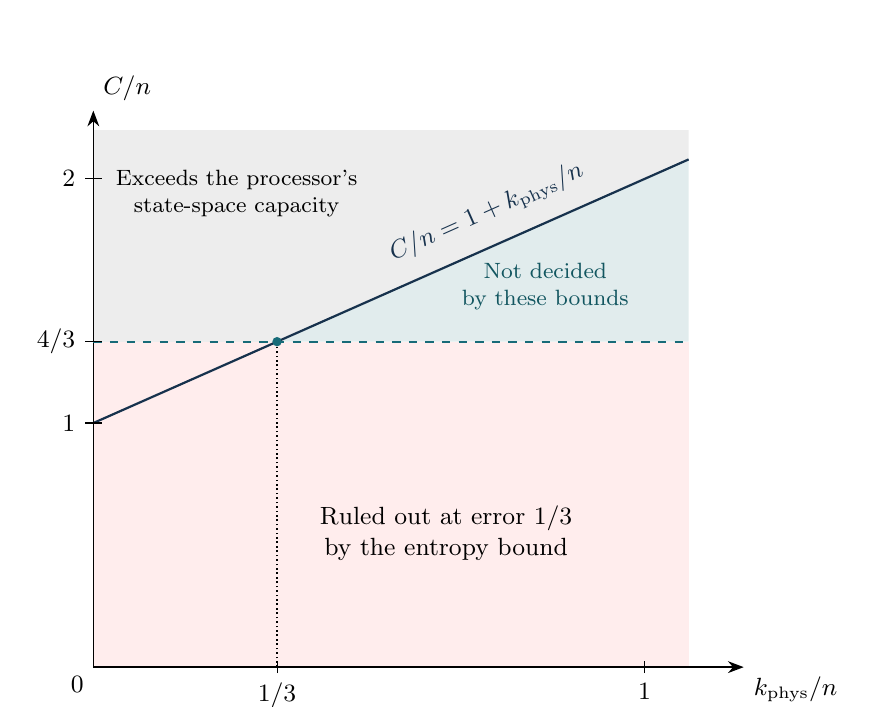
\begin{tikzpicture}[x=7cm,y=3.1cm,font=\small,>=Stealth]
  \fill[black!7] (0,1) -- (1.08,2.08) -- (1.08,2.2) -- (0,2.2) -- cycle;
  \fill[red!7] (0,0) rectangle (1.08,1.333333333);
  \fill[ReportTeal!13] (0.333333333,1.333333333) -- (1.08,1.333333333)
       -- (1.08,2.08) -- cycle;
  \draw[->,semithick] (0,0) -- (1.18,0) node[below right] {$k_{\rm phys}/n$};
  \draw[->,semithick] (0,0) -- (0,2.28) node[above right] {$C/n$};
  \draw[ReportNavy,thick] (0,1) -- (1.08,2.08);
  \node[ReportNavy,rotate=24,above] at (0.73,1.78)
       {$C/n=1+k_{\rm phys}/n$};
  \draw[ReportTeal,thick,dashed] (0,1.333333333) -- (1.08,1.333333333);
  \draw[densely dotted,semithick] (0.333333333,0) -- (0.333333333,1.333333333);
  \fill[ReportTeal] (0.333333333,1.333333333) circle (1.7pt);
  \node[align=center] at (0.64,0.55)
       {Ruled out at error $1/3$\\by the entropy bound};
  \node[align=center,ReportTeal!80!black,font=\footnotesize] at (0.82,1.56)
       {Not decided\\by these bounds};
  \node[align=center,font=\footnotesize] at (0.26,1.94)
       {Exceeds the processor's\\state-space capacity};
  \foreach \y/\lab in {1/1,1.333333333/{4/3},2/2}
    {\draw (-0.015,\y) -- (0.015,\y); \node[left] at (-0.015,\y) {$\lab$};}
  \foreach \x/\lab in {0.333333333/{1/3},1/1}
    {\draw (\x,-0.025) -- (\x,0.025); \node[below] at (\x,-0.025) {$\lab$};}
  \node[below left] at (0,0) {$0$};
\end{tikzpicture}
\caption{Necessary budgets for the weight-one, attenuation-$1/2$ task.
The whole processor has $n+k_{\rm phys}$ qubits, including every retained
record. The entropy condition $C\ge4n/3$ and dimension ceiling
$C\le n+k_{\rm phys}$ meet at $k_{\rm phys}=n/3$.
The teal region merely survives both inequalities; attainability there is
not established. This is not a diagram for a coherent-width convention
that exempts a classical history.}
\label{fig:joint-budget}
\end{figure}%
}
\begin{document}
\thispagestyle{plain}
\begin{center}
  {\color{ReportNavy}\LARGE\bfseries Coherent memory in Pauli channel learning\par}
  \vspace{0.5em}
  {\small Explanatory report}
\end{center}
\vspace{0.25em}
\noindent{\color{ReportTeal}\rule{\textwidth}{0.6pt}}
\vspace{0.3em}

\section{The question: how much of an unknown correlation can a probe see?}
A noisy quantum device can act very simply on every observable and still be difficult to learn. Imagine that an \(n\)-qubit device preserves one correlation, such as an \(X\) measurement on one site multiplied by a \(Z\) measurement on another, while randomizing the other correlations. If that correlation is specified before an experiment, the probe can be aligned with it. If the experiment must finish before the correlation is requested, one stored record must support many possible questions. That change in timing creates the learning problem studied here.

The principal resource is an outside quantum reference. At each call, the device acts on a register \(S\) of \(n\) qubits. At most \(k\) further qubits can remain coherent outside it. Their register is denoted by \(A\), so \(\dim A\leq 2^k\). A reference qubit can be entangled with a queried qubit and jointly measured afterward. It thereby makes more information about the error accessible than a local preparation and measurement.

The learning frontier concerns integers \(n\geq1\), \(0\leq k\leq n\), and \(1\leq w\leq n\), with \(0<\epsilon<1/3\) and \(0<\delta<1/2\). The accuracy and confidence are held fixed when interpreting the basic asymptotic statement. Individual upper bounds below are valid on the larger ranges explicitly stated with them.

The target weight \(w\) and the missing reference width \(n-k\) combine in the parameter
\begin{equation}
 R=\frac{w(n-k)}{n}.
 \label{eq:plmt-R}
\end{equation}
At fixed nontrivial accuracy and confidence, polynomially many channel calls suffice exactly when
\begin{equation}
 \boxed{R=O(\log n).}
 \label{eq:plmt-frontier}
\end{equation}
The statement allows the learner to preserve quantum states between calls, use feedback, and concatenate many calls before measuring. Each invocation is counted. The upper and lower bounds match this polynomial-versus-superpolynomial boundary, rather than an optimal numerical constant in the exponential rate.

The companion report \emph{Initial purity in quantum learning without resets} asks what changes when preparation is supplied only once. The shared weight-one, attenuation-\(1/2\) task then requires initial entropy deficit \(C\geq4n/3\), measured in bits, at decision error \(1/3\) for every finite query budget. We derive that obstruction after the width theorem, keeping the fresh-preparation and fixed-initialization contracts distinct.

\section{Pauli channels, late questions, and charged memory}
\subsection{Correlations and their binary labels}
A register is a collection of qubits treated as one system. An \(n\)-qubit register has a complex state space of dimension \(2^n\). Its density operator \(\rho\) is a positive semidefinite matrix with \(\operatorname{Tr}\rho=1\), where the trace is the sum of diagonal entries. Positivity makes all measurement probabilities nonnegative. A pure state has the form \(\rho=|\psi\rangle\langle\psi|\) for a unit vector \(|\psi\rangle\); a mixed state is a probability-weighted mixture of such matrices. For a Hermitian observable \(O\), the measurement mean is \(\operatorname{Tr}(O\rho)\).

Joined registers use a tensor-product state space. An uncorrelated state is \(\rho_S\otimes\rho_A\), but a general joint state need not factor in that way. The reduced state \(\rho_S=\operatorname{Tr}_A\rho_{SA}\) discards \(A\); this partial trace preserves the expectation of every observable acting only on \(S\). A quantum channel is a linear, trace-preserving transformation that remains positive when an untouched reference is adjoined. This reference-compatible positivity is the meaning of complete positivity.

A qubit has three Pauli observables, \(X,Y,Z\), each with measurement outcomes \(+1\) and \(-1\). The identity \(I\) ignores the site. An \(n\)-qubit Pauli observable is a tensor product of these four operators. Its support is the set of nonidentity factors; its weight is the number of those factors. For example, \(X\otimes I\otimes Z\) has weight two. Measuring its correlation means multiplying the \(X\) outcome on the first site by the \(Z\) outcome on the third.

It is useful to encode a Pauli by two bits per site. Let \(\mathbb F_2=\{0,1\}\), with addition modulo two, and write a label as \(v=(x,z)\in\mathbb F_2^{2n}\). A Hermitian phase convention is
\begin{equation}
 P_v=i^{\sum_jx_jz_j}\bigotimes_{j=1}^n X^{x_j}Z^{z_j}.
\end{equation}
At one site, the labels \((0,0),(1,0),(0,1),(1,1)\) represent \(I,X,Z,Y\), respectively. The phase in this definition makes each \(P_v\) Hermitian. It does not change a conjugation channel or a measured commutation sign.

For labels \(e,v\), define the binary symplectic pairing
\begin{equation}
 [e,v]=x_e\cdot z_v+z_e\cdot x_v \pmod 2.
\end{equation}
The operators commute when this bit is zero and anticommute when it is one:
\begin{equation}
 P_vP_eP_v=(-1)^{[e,v]}P_e,\qquad
 \operatorname{Tr}(P_eP_f)=d\,\mathbf 1_{\{e=f\}},\qquad d=2^n.
 \label{eq:plmt-pauli}
\end{equation}
Thus algebra becomes a recorded parity bit. The character
\(\chi_e(v)=(-1)^{[e,v]}\) is the corresponding sign.

A memoryless Pauli channel draws an error label from a distribution \(p(v)\) and applies its Pauli:
\begin{equation}
 \Lambda(\rho)=\sum_vp(v)P_v\rho P_v,\qquad p(v)\geq0,\quad\sum_vp(v)=1.
 \label{eq:plmt-channel}
\end{equation}
Memoryless means that every call implements the same channel without a hidden environment connecting different calls. It does not require the errors on different sites of one draw to be independent. They may be correlated across the entire device.

The Pauli basis diagonalizes this channel:
\begin{equation}
 \Lambda(P_e)=\lambda_eP_e,\qquad
 \lambda_e=\sum_vp(v)\chi_e(v)\in[-1,1].
 \label{eq:plmt-eigenvalue}
\end{equation}
The coefficient \(\lambda_e\) is a dimensionless input--output multiplier. An input mean \(\operatorname{Tr}(P_e\rho)\) becomes
\(\lambda_e\operatorname{Tr}(P_e\rho)\) after the channel. For instance, a one-qubit channel that applies \(I\) with probability \(0.9\) and \(X\) with probability \(0.1\) has \(\lambda_Z=0.8\): an \(X\) error reverses a \(Z\) outcome.

\subsection{One acquisition record, many possible requests}
The allowed target family is the complete Pauli ball
\begin{equation}
 \mathcal A_w=\{e:1\leq |e|\leq w\},\qquad
 M_w=\sum_{u=0}^w\binom nu3^u,\qquad 1\leq w\leq n.
 \label{eq:plmt-family}
\end{equation}
The identity coefficient is known to be one. Its term is included in \(M_w\) only for convenient counting; the hard channel alternatives below never use an identity spike.

The learner acquires a record before the particular label \(e\) is supplied. A decoder then returns an estimate \(\widehat\lambda_e\). For every allowed channel and every \(e\in\mathcal A_w\), the pointwise requirement is
\begin{equation}
 \Pr_\Lambda\{|\widehat\lambda_e-\lambda_e|\leq\epsilon\}\geq1-\delta.
 \label{eq:plmt-guarantee}
\end{equation}
Here \(\epsilon\) is an absolute coefficient error and \(\delta\) a failure probability. A simultaneous guarantee requires every estimate to be accurate on the same record with probability at least \(1-\delta\). It is stronger. The construction below achieves it, whereas the converse needs only \eqref{eq:plmt-guarantee}.

The target timing matters. If one Pauli is specified before acquisition, prepare the positive eigenstate of its local factors and measure the output parity. Each call gives a sign of mean \(\lambda_e\), so \(O(\epsilon^{-2}\ln(1/\delta))\) calls suffice without a reference. A polynomial-sized known list can also be measured coefficient by coefficient. The threshold concerns the whole support-and-axis family \(\mathcal A_w\), not every smaller list with maximum weight \(w\).

\subsection{The width contract}
At every actual invocation, all accessible coherent registers outside \(S\) are charged to \(A\). A classical history may be retained without a size restriction. Its state can be written
\begin{equation}
 \sum_hq_h|h\rangle\langle h|_H\otimes\omega^h_{SA},
 \qquad \dim S=2^n,\quad \dim A\leq2^k.
 \label{eq:plmt-cut}
\end{equation}
Known controls may depend on \(h\), move information between \(S\) and \(A\), measure, reset, and prepare new probes. The queried register \(S\) may itself preserve coherence between calls. Any implementation register still coherent outside \(S\) at a call counts toward \(k\).

The oracle is an ordinary use of \(\Lambda\otimes\operatorname{id}_A\). It supplies no inverse, controlled channel, channel environment, or purification of the channel action. In particular, an unlimited classical history is not an uncharged coherent controller.

The call budget \(T\) is worst-case: every execution uses at most \(T\) invocations. A coherent block of length \(L\) costs \(L\) calls even if it has one terminal measurement. An early halt is allowed. The lower-bound argument treats later query slots on a halted branch as inactive; it does not replace a deterministic budget with an expected count.

A fresh experiment is the restricted case in which a probe is prepared, the channel is used once, and the quantum output is completely measured before the next round. Preparation and measurement may still adapt to all earlier classical outcomes. This distinction will matter for the finite accuracy dependence.

\section{A partial-Bell construction}
\subsection{What a single experiment reveals}
One reference qubit paired with one queried qubit can identify a complete local Pauli error. Prepare
\[
 |\Phi^+\rangle=\frac{|00\rangle+|11\rangle}{\sqrt2}.
\]
The four states \((P_v\otimes I)|\Phi^+\rangle\), for the four local labels \(v\), are orthogonal. A Bell-basis measurement therefore returns the two error bits. This information is obtained through an ordinary channel call and a joint measurement; the device does not reveal its sampled error as an extra output.

At an unpaired site, choose an axis \(\alpha_i\in\{X,Y,Z\}\), prepare its positive eigenstate, and measure along that axis after the call. The sign is
\begin{equation}
 b_i=(-1)^{[\alpha_i,v_i]}.
\end{equation}
It reveals one commutation bit, rather than both local error bits.

A fresh partial-Bell experiment chooses a uniform \(k\)-element subset \(K\) of the \(n\) sites. It prepares Bell pairs on \(K\), and independent uniform local axes on the other sites. After one channel call, it measures every pair and every unpaired qubit. The classical record stores \(K\), the axes, the Bell labels, and the local signs. Each setting is chosen independently of the channel error.

\subsection{Compatibility with a later target}
Let the requested Pauli \(P_e\) have weight \(u\). Every paired site supplies both error bits, so it supports any local target axis. An unpaired active site supports the request only when its chosen axis agrees with that target factor. Define
\begin{equation}
 H_e=\mathbf 1\{\alpha_i=e_i\text{ for all }i\in\operatorname{supp}(e)\setminus K\}.
\end{equation}
On a compatible record, multiplying the appropriate Bell-label characters and local signs recovers
\begin{equation}
 Y_e=\chi_e(v)=(-1)^{[e,v]}.
\end{equation}
No independence between sites is used: conditional on the full error label \(v\), this equality is exact.

Let \(p_u=\Pr(H_e=1)\), which depends only on the target weight. If \(j\) target sites are paired, the other \(u-j\) axes must match. Grouping the random subsets by \(j\) gives
\begin{equation}
 p_u=
 \frac{1}{\binom nk}
 \sum_{j=0}^{u}\binom uj\binom{n-u}{k-j}3^{-(u-j)}.
 \label{eq:plmt-pu}
\end{equation}
Out-of-range binomial coefficients mean zero. Equivalently, if \(M\) is the number of unpaired active sites, then
\[
 p_u=\mathbb E_K3^{-M},\qquad \mathbb E_KM=\frac{u(n-k)}{n}.
\]
Because \(3^{-m}\) is convex,
\begin{equation}
 p_u\geq3^{-u(n-k)/n}.
 \label{eq:plmt-compatibility}
\end{equation}
Adding a target site can only multiply its conditional usability by \(1\) or \(1/3\). Permutation symmetry then shows that \(p_u\) is nonincreasing in \(u\), and \(p_w\geq3^{-R}\).

This explains the constructive meaning of \(R\). A weight-\(u\) target has, on average, \(u(n-k)/n\) active sites without references. Each is a possible axis mismatch. The converse must show that this mechanism reflects a universal width obstruction, rather than just a weakness of these particular probes.

\subsection{Variance, rather than range alone, sets the sample cost}
Use the one-record estimate
\begin{equation}
 X_e=\frac{H_eY_e}{p_u},
\end{equation}
implemented as zero when the record is unusable. Settings are independent of the error draw. Consequently
\begin{equation}
 \mathbb E X_e=\lambda_e,\qquad
 \mathbb E X_e^2=\frac1{p_u},\qquad
 \operatorname{Var}(X_e)\leq\frac1{p_u}.
 \label{eq:plmt-moments}
\end{equation}
The normalization compensates for missing records. It can make an individual sample larger than one even though the coefficient being estimated lies in \([-1,1]\).

For \(T\) independent calls, average the \(X_e\)'s. Their centered magnitude is at most \(2/p_u\). Bernstein's concentration inequality therefore gives
\begin{equation}
 \Pr\{|\widehat\lambda_e-\lambda_e|\geq\epsilon\}
 \leq
 2\exp\!\left[-\frac{T\epsilon^2p_u}{2+4\epsilon/3}\right].
 \label{eq:plmt-bernstein}
\end{equation}
For \(0<\epsilon\leq1\), the denominator is below four. A range-only bound would unnecessarily use \(p_u^{-2}\); retaining the second moment gives \(p_u^{-1}\).

For any \(0<\epsilon\leq1\) and \(0<\delta<1\), a union bound over the targets proves the simultaneous guarantee with
\begin{equation}
 T=
 \left\lceil4\epsilon^{-2}p_w^{-1}
 \ln\frac{2M_w}{\delta}\right\rceil
 \leq
 \left\lceil4\epsilon^{-2}3^R
 \ln\frac{2M_w}{\delta}\right\rceil.
 \label{eq:plmt-upper}
\end{equation}
Here and below, \(\ln\) denotes the natural logarithm. Estimates for different targets may be correlated because they use the same record; the union bound requires no independence between them.

Each call uses \(n\) queried qubits, \(k\) reference qubits, and \(O(n)\) ideal local or Bell operations. Its record occupies \(O(n)\) bits, hence \(O(nT)\) bits over acquisition. One later coefficient can be decoded by scanning the records in \(O(nT)\) elementary operations with polynomial-bit arithmetic. The exact probability \eqref{eq:plmt-pu} is a computable rational number of polynomial bit length. There is no quantum random-access memory or exponentially large normalization table. Printing the entire family, however, must pay for its output length.

\subsection{A complete two-qubit example}
Take \(n=2\), \(k=1\), and a later request \(P=X\otimes Z\). Pair the first site with the reference and choose the \(Z\) axis on the second. Prepare \(|\Phi^+\rangle_{S_1A}|0\rangle_{S_2}\). The record contains
\[
 y=(x_1,z_1,x_2),
\]
because the Bell measurement reveals \((x_1,z_1)\) and the second measurement reveals the \(Z\)-flip bit \(x_2\). The requested sign is \((-1)^{z_1+x_2}\). If instead site two is paired, the unpaired first site must use \(X\), and the sign is recovered in the same way.

For a weight-two target, either choice of paired site leaves one required axis, so \(p_2=1/3\). For a weight-one target,
\[
 p_1=\frac12+\frac12\frac13=\frac23.
\]
The weight-two sample is \(3Y_e\) on usable settings and zero otherwise. It has mean \(\lambda_e\), second moment three, and variance \(3-\lambda_e^2\). If every error commutes with the requested Pauli, samples are three with probability \(1/3\) and zero otherwise: the mean is one. Three records do not by themselves establish a useful confidence interval; this example explains the record and normalization, while \eqref{eq:plmt-bernstein} supplies the statistical guarantee.

At the endpoints, \(k=n\) gives \(p_u=1\), ordinary Bell sampling. With \(k=0\), \(p_u=3^{-u}\), random local-axis sampling. Random partial pairing interpolates between them.

\section{A universal analytic limitation from reference rank}
\subsection{Why rank enters a physical width bound}
For a pure probe \(|\psi\rangle_{SA}\), its Schmidt decomposition has at most \(\dim A\) terms:
\[
 |\psi\rangle=\sum_{j=1}^{r}\sqrt{\mu_j}|u_j\rangle_S|v_j\rangle_A,
 \qquad r\leq2^k.
\]
Thus the system marginal \(\rho_S\) has rank at most \(2^k\). A mixed probe can have a higher-rank system marginal. The proof will decompose it into pure states \emph{within the actual registers}, rather than adding an uncharged purification.

Low rank restricts the response averaged over unknown Pauli directions. We need one bound for the average quantum-output response of persistent coherent strategies and another for the squared likelihood response of fresh experiments. Both will follow from the same rank-dependent suppression factor.

\subsection{A low-weight prior is an averaging device}
For \(0\leq x\leq1\), introduce the normalized product distribution
\begin{equation}
 \nu_x(e)=\frac{x^{|e|}}{(1+3x)^n},\qquad
 t=\frac{1-x}{1+3x},\qquad
 \gamma=\frac{1-t}{1+t}=\frac{2x}{1+x}.
 \label{eq:plmt-prior}
\end{equation}
A site is identity with probability \(1/(1+3x)\), and each nonidentity axis has probability \(x/(1+3x)\). For any fixed Pauli label \(b\),
\[
 \mathbb E_{\nu_x}\chi_e(b)=t^{|b|}.
\]
The identity contributes a positive sign; a nonidentity local label commutes with itself and anticommutes with the other two axes.

For \(0\leq s\leq1\), let \(\Delta_s(F)=sF+(1-s)\operatorname{Tr}(F)I_2/2\) be a one-qubit depolarizing map, and set \(\mathcal T_s=\Delta_s^{\otimes n}\). Then
\begin{equation}
 \mathcal T_s(P_b)=s^{|b|}P_b,\quad
 \mathcal T_s\mathcal T_u=\mathcal T_{su},\quad
 \mathbb E_{\nu_x}P_eFP_e=\mathcal T_t(F).
 \label{eq:plmt-averaging}
\end{equation}
These maps average the proof's Pauli directions. They are not additional noise imposed on the learner's reference.

For a matrix \(F\), write \(F^\dagger\) for its conjugate transpose. The Schatten norm
\(\|F\|_p=(\operatorname{Tr}|F|^p)^{1/p}\), with
\(|F|=\sqrt{F^\dagger F}\), is the \(p\)-norm of its singular values. The dimension-normalized version is
\(\|F\|_{p,\mathrm{av}}=(d^{-1}\operatorname{Tr}|F|^p)^{1/p}\).
The normalization gives \(I_d\) norm one. For rank \(r\) and \(1\leq p\leq2\), the ordinary finite-dimensional comparison of singular values yields
\begin{equation}
 \|F\|_{p,\mathrm{av}}
 \leq(r/d)^{1/p-1/2}\|F\|_{2,\mathrm{av}}.
 \label{eq:plmt-rank}
\end{equation}
The \(p=2\) norm is the Hilbert--Schmidt or Frobenius norm, also written
\(\|F\|_F=\|F\|_2=(\operatorname{Tr}F^\dagger F)^{1/2}\).

We use an established tensor-product hypercontractive inequality, explicitly as an analytic input:
\[
 \|\mathcal T_s(F)\|_{q,\mathrm{av}}\leq\|F\|_{p,\mathrm{av}}
 \quad\text{if}\quad
 1<p\leq q,\quad
 0\leq s\leq\sqrt{\frac{p-1}{q-1}}.
\]
It applies to arbitrary complex matrices, including non-Hermitian ones. With \(q=2\), \(p=1+t\), and \(s=\sqrt t\), combine it with \eqref{eq:plmt-rank} and square:
\begin{equation}
 \|\mathcal T_{\sqrt t}(F)\|_{2,\mathrm{av}}^2
 \leq(r/d)^\gamma\|F\|_{2,\mathrm{av}}^2.
 \label{eq:plmt-hyper-rank}
\end{equation}
At \(t=0\), the same endpoint follows directly from
\(|d^{-1}\operatorname{Tr}F|\leq d^{-1}\operatorname{Tr}|F|\).
At \(t=1\), the exponent is zero and the bound is an identity. This makes the complete interval precise.

\subsection{The complex likelihood response}
For a nonzero complex matrix \(C\) of rank \(r\), define
\begin{equation}
 G_e(C)=
 \frac{\operatorname{Tr}(P_eCP_eC^\dagger)}
 {\operatorname{Tr}(CC^\dagger)}.
\end{equation}
Although \(C\) need not be Hermitian, this response is real. To see why, expand in the orthogonal Pauli basis and define probability weights
\[
 q_b=\frac{|\operatorname{Tr}(P_bC)|^2}
 {d\operatorname{Tr}(CC^\dagger)},\qquad \sum_bq_b=1.
\]
Equation \eqref{eq:plmt-pauli} gives
\[
 G_e(C)=\sum_bq_b\chi_e(b),\qquad |G_e(C)|\leq1.
\]
Averaging its square produces
\[
 \mathbb E_{\nu_x}G_e(C)^2
 =\sum_{b,c}q_bq_ct^{|b+c|}.
\]
For each fixed \(c\), multiplication by \(P_c\) shifts Pauli labels without changing rank or singular values. Parseval's identity therefore gives
\[
 \sum_bq_bt^{|b+c|}
 =
 \frac{\|\mathcal T_{\sqrt t}(P_cC)\|_{2,\mathrm{av}}^2}
 {\|C\|_{2,\mathrm{av}}^2}.
\]
Every such row is bounded by \((r/d)^\gamma\) using \eqref{eq:plmt-hyper-rank}. Averaging the rows proves
\begin{equation}
 \boxed{\mathbb E_{\nu_x}G_e(C)^2\leq(r/d)^\gamma.}
 \label{eq:plmt-G}
\end{equation}
\subsection{The quantum-output response}
For a density matrix \(\rho\) of rank \(r\), define
\[
 f_e(\rho)=\|\sqrt\rho P_e\sqrt\rho\|_1.
\]
This is the unsquared, or root, fidelity between \(\rho\) and \(P_e\rho P_e\). Schatten Holder's inequality with exponents \(4,2,4\), applied to
\[
 \sqrt\rho P_e\sqrt\rho
 =\rho^{1/4}(\rho^{1/4}P_e\rho^{1/4})\rho^{1/4},
\]
implies
\[
 f_e(\rho)^2\leq
 \operatorname{Tr}(\sqrt\rho P_e\sqrt\rho P_e).
\]
The right-hand side is nonnegative: it is the squared Hilbert--Schmidt norm of \(\rho^{1/4}P_e\rho^{1/4}\). Average using \eqref{eq:plmt-averaging}, put \(F=\sqrt\rho\), and use self-adjointness and the semigroup property:
\begin{align}
 \mathbb E_{\nu_x}f_e(\rho)^2
 &\leq \operatorname{Tr}(F\mathcal T_t(F))\\
 &=d\|\mathcal T_{\sqrt t}(F)\|_{2,\mathrm{av}}^2
 \leq(r/d)^\gamma.
 \label{eq:plmt-f}
\end{align}
The final equality of normalization uses \(\operatorname{Tr}(F^\dagger F)=1\). Both \eqref{eq:plmt-G} and \eqref{eq:plmt-f} thus give the suppression
\[
 B_x=2^{-(n-k)\gamma}
\]
whenever the relevant rank is at most \(2^k\).

\subsection{Restricting the prior to physical targets}
The product prior includes the identity and labels above weight \(w\). For \(0<x\leq1\), the physical hidden label can follow \(\nu_x\) conditioned on \(\mathcal A_w\). The endpoint \(x=0\) remains an algebraic endpoint of the unconditioned moment bounds, but cannot be conditioned this way because the family then has zero probability. Write \(p_{\mathcal A}(x)=\nu_x(\mathcal A_w)\) and \(\pi_x=\nu_x(\cdot\mid\mathcal A_w)\). For any nonnegative squared response, discarding terms outside that family and renormalizing gives
\begin{equation}
 \mathbb E_{\pi_x}g_e^2
 \leq \frac{B_x}{p_{\mathcal A}(x)},
 \qquad
 \mathbb E_{\pi_x}|g_e|
 \leq\sqrt{\frac{B_x}{p_{\mathcal A}(x)}}.
 \label{eq:plmt-conditioning}
\end{equation}
The second inequality is Cauchy--Schwarz under the conditioned probability measure. In the following width lower bounds, \(\mathbb E_e\) denotes this conditioned-prior average unless another prior is specified.

Choose
\begin{equation}
 x_*=\frac{w}{3(2n-w)},\qquad
 \kappa=\frac{w}{3n-w}.
 \label{eq:plmt-kappa}
\end{equation}
The random weight under this prior is
\(W\sim\operatorname{Bin}(n,w/(2n))\), so its mean is \(w/2\), and
\(\gamma=\kappa\). Importantly,
\begin{equation}
 p_{\mathcal A}(x_*)=\Pr(1\leq W\leq w)\geq\frac14.
 \label{eq:plmt-mass}
\end{equation}
For \(w=1\), its exact value is
\(\frac12(1-\frac1{2n})^{n-1}\geq(n+1)/(4n)\).
For \(w=2\), the zero probability is at most \(e^{-1}\), while
\(\Pr(W\geq3)\leq1/3\), giving \(p_{\mathcal A}(x)\geq2/3-e^{-1}>1/4\).
For \(w\geq3\), the zero probability is at most \(e^{-3/2}\) and
\(\Pr(W>w)\leq w/[2(w+1)]\leq1/2\), again giving the claim.
From now on use \(x=x_*\) unless a different endpoint prior is specified. The identity is therefore excluded without an exponentially small conditioning cost. The suppression becomes \(B_{x_*}=2^{-\kappa (n-k)}\).

\section{The coherent lower bound counts every call}
To lower-bound learning, consider depolarization and a channel with one coefficient equal to \(3\epsilon\). Requesting that coefficient after acquisition separates the two cases. We bound the change caused by one invocation, then sum over all invocations while retaining feedback and stored quantum states.
\subsection{Physical alternatives}
Against complete depolarization
\[
 \Dep(F)=\frac{\operatorname{Tr}F}{d}I_d,
\]
consider a nonidentity label \(e\) and amplitude \(0<\lambda\leq1\):
\begin{equation}
 \mathcal E_{e,\lambda}(F)=
 \Dep(F)+\frac{\lambda}{d}\operatorname{Tr}(P_eF)P_e.
 \label{eq:plmt-spike}
\end{equation}
This is a physical Pauli channel. Its error probabilities are
\[
 p^{(e,\lambda)}(v)=4^{-n}[1+\lambda\chi_e(v)].
\]
They are nonnegative, and sum to one because a nonidentity character has zero average. The Pauli eigenvalues are one at the identity, \(\lambda\) at \(e\), and zero elsewhere. An identity label cannot be used in this formula as a spike: the extra term would change trace preservation.

\subsection{One changed invocation}
For an input state \(\omega_{SA}\), define an operator on the reference,
\[
 B_e(\omega)=
 \operatorname{Tr}_S[(P_e\otimes I_A)\omega].
\]
The difference of the two outputs is
\[
 [(\mathcal E_{e,\lambda}-\Dep)\otimes\operatorname{id}_A](\omega)
 =\frac{\lambda}{d}P_e\otimes B_e(\omega).
\]
Since \(\|P_e\|_1=d\), its trace norm is
\(\lambda\|B_e(\omega)\|_1\). For a pure input, the Schmidt representation shows that the nonzero block of \(B_e(\omega)\) is a transpose of the corresponding block of \(\sqrt{\rho_S}P_e\sqrt{\rho_S}\). Transposition preserves singular values. Equation \eqref{eq:plmt-f} therefore bounds its squared norm by \(B_x\) after averaging.

For a mixed input, decompose \(\omega=\sum_ju_j|\psi_j\rangle\langle\psi_j|\) within the actual \(S\otimes A\). Trace-norm convexity and then Jensen's inequality give
\[
 \|B_e(\omega)\|_1^2
 \leq\sum_ju_j\|B_e(|\psi_j\rangle\langle\psi_j|)\|_1^2.
\]
The same second-moment bound follows without assuming a low-rank mixed system marginal. The classical blocks in \eqref{eq:plmt-cut} are handled by the same convexity argument. Their number does not enter.

Write \(D_{\mathrm{tr}}(\rho,\sigma)=\frac12\|\rho-\sigma\|_1\). It bounds the change in probability of any final measurement event and contracts under a common completely positive trace-preserving map. For an input independent of the hidden label, \eqref{eq:plmt-conditioning} gives the mean one-call distance bound
\begin{equation}
 \mathbb E_eD_{\mathrm{tr}}(\text{spike output},\text{null output})
 \leq\frac{\lambda}{2}\sqrt{\frac{B_x}{p_{\mathcal A}(x)}}.
 \label{eq:plmt-onecall}
\end{equation}

\subsection{Why adaptivity does not invalidate the average}
The input during the actual spike execution can depend on \(e\). Applying \eqref{eq:plmt-onecall} directly to such a state would be invalid. Instead compare mathematical executions with increasing null prefixes. Execution \(j\) uses the null channel in its first \(j\) query slots and the spike afterward. Neighboring executions have the same null prefix, so their input at the differing call is independent of \(e\). Their subsequent operations are the same physical map for each fixed \(e\), even if that map includes further spike calls and feedback. Contraction applies to that common suffix.

The triangle inequality over all \(T\) slots yields, for the full acquisition outputs \(\sigma_0^{(e)}\) and \(\sigma_T\),
\begin{equation}
 \mathbb E_eD_{\mathrm{tr}}(\sigma_0^{(e)},\sigma_T)
 \leq\frac{T\lambda}{2}\sqrt{\frac{B_x}{p_{\mathcal A}(x)}}.
 \label{eq:plmt-hybrid}
\end{equation}
On a halted classical branch, later slots are inactive and contribute zero. The active probabilities sum to at most one, which preserves the convex bound. This is why a worst-case budget and ordinary early stopping are compatible with the argument.

Set \(\lambda=3\epsilon<1\). Once the label is revealed, threshold the estimated coefficient at \(3\epsilon/2\). Accurate null estimates are at most \(\epsilon\); accurate positive-spike estimates are at least \(2\epsilon\). Thus a valid learner gives a test whose probability of accepting the alternative differs by at least \(1-2\delta\). This holds for every label separately, even when its final measurement depends on that label. Therefore each output distance is at least \(1-2\delta\).

Combining with \eqref{eq:plmt-hybrid} and using \eqref{eq:plmt-kappa}--\eqref{eq:plmt-mass} proves
\begin{equation}
 \boxed{T_{\mathrm{coherent}}\geq
 \frac{1-2\delta}{3\epsilon}
 2^{\,w(n-k)/[2(3n-w)]}.}
 \label{eq:plmt-coherent-lower}
\end{equation}
The proof permits quantum information to survive for arbitrarily many calls. Its inverse-accuracy factor is \(\epsilon^{-1}\), not \(\epsilon^{-2}\).

For the full family \(w=n\), one can instead take the uniform Pauli prior \(x=1\). Its nonidentity mass is \(1-4^{-n}\) and \(\gamma=1\), giving the stronger endpoint
\[
 T_{\mathrm{coherent}}\geq
 \frac{2(1-2\delta)\sqrt{1-4^{-n}}}{3\epsilon}\,2^{(n-k)/2}.
\]
The uniform finite expression \eqref{eq:plmt-coherent-lower} is convenient across all weights, but is not the strongest available expression at this endpoint.

The exponent in \eqref{eq:plmt-coherent-lower} is
\(R/[2(3-w/n)]\), between \(R/6\) and \(R/4\).
Meanwhile \(M_w\leq4^n\), so the confidence logarithm in
\eqref{eq:plmt-upper} is at most \(O(n+\ln(1/\delta))\).
These inequalities prove \eqref{eq:plmt-frontier}. In particular, if
\(R/\log n\to\infty\), every allowed coherent learner needs superpolynomially many calls.

\section{Why fresh experiments give a sharper accuracy factor}
A classical transcript permits a different argument. Use a sign \(s\in\{-1,+1\}\) chosen once at the start, and let
\(\mathcal E_{e,s\lambda}=\Dep+s\lambda\,\operatorname{Tr}(P_e\,\cdot)P_e/d\), with \(0<\lambda<1\). Its probabilities
\(4^{-n}[1+s\lambda\chi_e(v)]\) remain physical.

Fix a history and one fresh experiment. For a pure probe and rank-one measurement effect, write their system-by-reference amplitude matrices as \(\Psi\) and \(M\):
\[
 |\psi\rangle=\sum_{i,\alpha}\Psi_{i\alpha}|i\rangle|\alpha\rangle,
 \qquad |m\rangle=\sum_{i,\alpha}M_{i\alpha}|i\rangle|\alpha\rangle .
\]
Here \(i=1,\ldots,d\), \(\alpha=1,\ldots,r\), \(r\leq2^k\), and \(\|\Psi\|_F=1\). The effect vector need not be normalized. The contraction \(C=M\Psi^\dagger\) has rank at most \(r\). Direct substitution into the channel gives
\begin{equation}
 q_{\Dep}=\frac{\|C\|_F^2}{d},\qquad
 \frac{q_{e,s}}{q_{\Dep}}=1+s\lambda G_e(C)
 \quad(q_{\Dep}>0).
 \label{eq:plmt-likelihood}
\end{equation}
For example, the identity
\(\langle m|A\otimes B|m\rangle=\operatorname{Tr}(M^\dagger A M B^{\mathsf T})\),
together with the probe's reference block
\((\operatorname{Tr}_S[(P_e\otimes I)|\psi\rangle\langle\psi|])^{\mathsf T}
=\Psi^\dagger P_e\Psi\),
produces the numerator in \(G_e\). The transpose is a basis convention, not an extra physical operation.

Mixed preparations and general measurement effects are positive sums of these elementary pairs. Their normalized null weights express the complete outcome response \(g_e\) as a convex combination of \(G_e\)'s. Those weights are independent of \(e,s\), so \(|g_e|\leq1\) and
\(\mathbb E_e g_e^2\leq B_x/p_{\mathcal A}(x)\).
If a null outcome has probability zero, every positively weighted elementary pair has \(C=0\), hence zero signal as well. No missing alternative-only outcome invalidates the likelihood ratio.

For a transcript \(z=(z_1,\ldots,z_T)\), the likelihood ratio of a whole execution is a product,
\[
 L_{e,s}(z)=\prod_{\ell=1}^T
 (1+s\lambda g_{e,\ell}(z_{\leq\ell})).
\]
The sign is fixed across the entire execution. Averaging the two complete transcript laws, rather than independently resampling the sign at each call, gives
\[
 \overline L_e=\frac{L_{e,+}+L_{e,-}}2
 \geq\prod_{\ell=1}^T\sqrt{1-\lambda^2g_{e,\ell}^2}
 \geq1-\lambda^2\sum_{\ell=1}^Tg_{e,\ell}^2.
\]
The first inequality is arithmetic--geometric mean; the second follows from
\(\sqrt{1-u}\geq1-u\) and \(\prod_\ell(1-u_\ell)\geq1-\sum_\ell u_\ell\).
Total variation equals the null expectation of \([1-\overline L_e]_+\).
Under the null, every history is independent of the hidden label, including the settings adaptively selected at that history. Averaging the node bound therefore yields
\[
 \mathbb E_e\operatorname{TV}
 \left(Q_0,\frac{Q_{e,+}+Q_{e,-}}2\right)
 \leq\frac{T\lambda^2B_x}{p_{\mathcal A}(x)}.
\]
This step never replaces the posterior of a spike execution by the original prior.

Choose \(\lambda=3\epsilon\) and accept either signed alternative when
\(|\widehat\lambda_e|>3\epsilon/2\). Successful estimation requires total variation at least \(1-2\delta\). Consequently
\begin{equation}
 \boxed{T_{\mathrm{fresh}}\geq
 \frac{1-2\delta}{36\epsilon^2}
 2^{\,w(n-k)/(3n-w)}.}
 \label{eq:plmt-fresh-lower}
\end{equation}
This is sharper than the coherent bound in accuracy and exponent, but it requires complete measurement between experiments. The two finite rates must not be interchanged.

\section{A one-bit test with efficient classical processing}
\subsection{The exact preserved-correlation promise}
Learning coefficients is not necessary if the only desired answer is whether one hidden correlation exists. Fix a known \(0<\tau\leq1\). The promise is either
\begin{equation}
 \Gamma_0=(1-\tau)\operatorname{id}+\tau\Dep,
 \qquad
 \Gamma_e=(1-\tau)\operatorname{id}+\tau\mathcal E_{e,1},
 \quad e\in\mathcal A_w.
 \label{eq:plmt-detect-promise}
\end{equation}
The hidden label is never supplied. The tester must distinguish the null from every alternative with error at most \(\delta\).

Under the null, every nonidentity coefficient is \(1-\tau\). Under the alternative, the distinguished coefficient is exactly one, while all others remain \(1-\tau\). At \(\tau=1\), the alternative error label is uniform on the hyperplane
\[
 \mathcal H_e=\{v:[e,v]=0\}.
\]
This has \(2^{2n-1}\) labels. Given \(e\), it can be sampled with \(2n-1\) random bits and one parity equation, so the physical family has a succinct description. The learner is not given that description.

The channel \(\mathcal E_{e,1}\) also measures the parity projectors
\(\Pi_\pm=(I\pm P_e)/2\) and prepares \(2\Pi_\pm/d\) after the corresponding outcome. It is entanglement breaking, even though a reference can help learn its hidden axis. The identity mixture for \(\tau<1\) need not be entanglement breaking.

For orientation, the full diamond norm obeys
\(\|\Gamma_i-\operatorname{id}\|_\diamond\leq2\tau\) and
\(\|\Gamma_e-\Gamma_0\|_\diamond=\tau\). The diamond norm allows an arbitrary reference when defining channel distinguishability. Its entangled witness establishes a norm identity; it does not grant the width-constrained tester such a reference.

The direct hybrid from the previous section, now with null \(\Gamma_0\) and amplitude \(\tau\), gives
\begin{equation}
 T\geq\frac{1-2\delta}{\tau}
 2^{\,w(n-k)/[2(3n-w)]}.
 \label{eq:plmt-det-lower}
\end{equation}
This is a converse for the one-bit task itself. It does not assume that detection is as hard as learning all coefficients.
For \(w=n\), the same uniform-prior refinement replaces its right-hand side by
\(2(1-2\delta)\sqrt{1-4^{-n}}\,2^{(n-k)/2}/\tau\).

\subsection{An unknown parity becomes missing rank}
Fix one partial-Bell setting and repeat it. Its outcomes form a linear syndrome
\[
 y=Av\in\mathbb F_2^m,\qquad m=n+k.
\]
Each paired site reveals two coordinate bits and each unpaired site one commutation bit. The \(m\) rows of the binary matrix \(A\) are independent. If the target character row \(\ell_e:v\mapsto[e,v]\) lies in the row space of \(A\), the setting is compatible. This is exactly the earlier local-axis compatibility condition.

Under the null, \(y\) has law
\((1-\tau)\delta_0+\tau\,\operatorname{Uniform}(\mathbb F_2^m)\).
In a compatible alternative setting, some nonzero row \(c\) obeys
\(cA=\ell_e\), and every sample satisfies \(cy=0\). In an incompatible setting, projection of the hidden hyperplane onto the syndrome space is surjective, and the syndrome law equals the null law. The identity branch adds a zero syndrome in either case and preserves every homogeneous constraint.

Draw \(J\) settings and repeat each for \(L\) calls. Stack the raw syndrome rows from each block. Output alternative if any block has binary rank below \(m\). Rank counts independent directions, not distinct observed strings. The algorithm finds a missing parity without enumerating candidate Paulis or identifying the hidden label.

A weight-\(u\) alternative misses compatibility in all \(J\) settings with probability at most \(e^{-Jp_u}\). Under the null, any fixed nonzero parity vanishes on a sample with probability \(1-\tau/2\). A union bound over the nonzero parities gives
\[
 \Pr_{\Gamma_0}\{\operatorname{rank}<m\}
 \leq(2^m-1)(1-\tau/2)^L
 \leq2^m e^{-\tau L/2}.
\]
Thus the finite choices
\begin{equation}
 J=\left\lceil3^R\ln\frac2\delta\right\rceil,\qquad
 L=\left\lceil\frac2\tau
 \left(m\ln2+\ln\frac{2J}{\delta}\right)\right\rceil,
 \qquad T=JL
 \label{eq:plmt-JL}
\end{equation}
control both error types. Streaming Gaussian elimination uses \(O(m^2)\) stored classical bits and \(O(Tm^2)\) bit operations. This is polynomial processing in the polynomial-call regime.

For the two-qubit example, \(m=3\), \(R=1\), \(\delta=1/10\), and \(\tau=1\), these sufficient formulas give \(J=9\), \(L=15\), and \(T=135\). With hidden \(X\otimes Z\), the compatible setting previously described satisfies \(y_2+y_3=0\). Its rows \((1,0,0),(0,1,1),(1,1,1)\) have rank two: the third is the binary sum of the first two. A null block can have deficient rank by chance, but its probability is at most \(7\,2^{-L}\). At \(\tau=1/4\), the same prescription gives \(L=59\) and \(T=531\); rare nonzero syndromes require more repetitions.

Together with \eqref{eq:plmt-det-lower}, the construction establishes
\begin{equation}
 \boxed{R+\log(1/\tau)=O(\log n)}
 \label{eq:plmt-det-frontier}
\end{equation}
as the criterion for polynomial query cost and polynomial total processing at fixed nontrivial confidence. The base of the logarithm does not change this asymptotic criterion.

Exact preservation is essential to the rank algorithm. If the hidden coefficient is \(1/2\), the relevant parity can be violated and raw rank need not remain deficient. An identity mixture with \(\tau=1/2\) still preserves the hidden coefficient at one; it is not an attenuated spike with retained coefficient \(1/2\).

\section{Weak noise: precision determines whether rare events matter}
Consider an unknown channel
\begin{equation}
 \widetilde\Lambda=(1-\tau)\operatorname{id}+\tau\Lambda,
 \qquad 0<\tau\leq1,
 \label{eq:plmt-weak-channel}
\end{equation}
with known \(\tau\) and otherwise arbitrary Pauli channel \(\Lambda\). Its coefficients satisfy
\(\widetilde\lambda_e=1-\tau+\tau\lambda_e\in[1-2\tau,1]\).
The branch is not observed; the actual probability of a nonidentity error can be smaller than \(\tau\).

The original estimator fluctuates even on the identity channel because compatibility is random. Centering at the known identity response removes that avoidable fluctuation. On the same partial-Bell record use
\[
 Z_e=1-\frac{H_e(1-Y_e)}{p_u}.
\]
It is one on every unusable record and whenever the actual error is identity. Put
\(\Delta_e=1-\widetilde\lambda_e\in[0,2\tau]\). Since
\((1-Y_e)^2=2(1-Y_e)\),
\begin{equation}
 \mathbb E Z_e=\widetilde\lambda_e,\qquad
 \operatorname{Var}(Z_e)=\frac{2\Delta_e}{p_u}-\Delta_e^2
 \leq\frac{4\tau}{p_u}.
\end{equation}
The centered magnitude is at most \(2/p_u\). Bernstein concentration and a union bound, now for \(0<\epsilon<\tau/3\), give the sufficient count
\begin{equation}
 T_{\mathrm{fresh}}\leq
 \left\lceil9\tau\epsilon^{-2}3^R
 \ln\frac{2M_w}{\delta}\right\rceil.
 \label{eq:plmt-weak-upper}
\end{equation}
The variance scales with the rate of rare informative events.

The matching scale in the lower prefactor requires more than rescaling the eigenvalue displacement. At a weak-null history let
\(q_0(y)=(1-\tau)q_{\operatorname{id}}(y)+\tau q_{\Dep}(y)\).
The signed alternatives have likelihood
\[
 \frac{\widetilde q_{e,s}(y)}{q_0(y)}
 =1+s\lambda h_e(y),\qquad
 h_e(y)=\frac{\tau q_{\Dep}(y)}{q_0(y)}g_e(y).
\]
Zero-probability outcomes are omitted as before; set \(h_e=0\) when
\(q_{\Dep}=0<q_0\). The inequality \(q_0\geq\tau q_{\Dep}\) gives
\[
 \sum_yq_0(y)\mathbb E_eh_e(y)^2
 \leq\frac{\tau B_x}{p_{\mathcal A}(x)}.
\]
Apply the signed-transcript argument with \(\lambda=3\epsilon/\tau<1\).
It yields
\begin{equation}
 T_{\mathrm{fresh}}\geq
 \frac{(1-2\delta)\tau}{36\epsilon^2}\,2^{\kappa (n-k)},
 \qquad
 T_{\mathrm{coherent}}\geq
 \frac{1-2\delta}{3\epsilon}\,2^{\kappa (n-k)/2}.
 \label{eq:plmt-weak-lower}
\end{equation}
The factor \(\tau\) in the fresh bound comes from an outcome-weighted second moment under the weak null. No mixture flag or expected-query shortcut is assumed.

For fixed relative accuracy \(\epsilon=\alpha\tau\), \(0<\alpha<1/3\), both upper and lower call bounds contain a \(1/\tau\) factor. Equations
\eqref{eq:plmt-weak-upper}--\eqref{eq:plmt-weak-lower} establish the same criterion \eqref{eq:plmt-det-frontier} for learning in both models. The variance is proportional to \(\tau\), while the required squared error is proportional to \(\tau^2\); their ratio explains the upper factor \(1/\tau\), and the converse shows that it cannot be uniformly avoided.

Absolute accuracy can be a different question. If \(\epsilon\geq\tau\), returning the known midpoint \(1-\tau\) needs no calls at all. For example, \(\tau=1/4\) and absolute error \(1/4\) are trivial, whereas relative factor \(\alpha=1/4\) asks for error \(1/16\). These weak channels may have rare global correlated errors. Small diamond distance to the identity does not imply independent local errors or a sparse local noise generator.

\section{A second resource: initial purity without replenishment}
\subsection{The shared task and the changed operating contract}
The width model permits resets, freshly prepared probes, and a growing classical record. To ask whether that preparation supply can be removed, fix one initialized processor \(SA\). Every protected register and retained record now belongs to the finite register \(A\). Known controls on the complete processor are unital:
\[
 \mathcal C_t(I_{SA})=I_{SA}.
\]
They are also completely positive and trace preserving. A unitary or nonselective dephasing is allowed. A reset to a pure state is not. A measurement record is permitted only through a complete implementation respecting this same initialized-memory and unital-control contract. There is no free fresh record after a measurement.

The null is complete depolarization of \(S\). The alternative retains one of the \(3n\) weight-one Paulis at coefficient \(1/2\). Write the label as \(e=(i,\alpha)\), where \(i=1,\ldots,n\) and \(\alpha\in\{X,Y,Z\}\). On the complete processor define
\begin{align}
 Q_0(F)&=\frac{I_S}{d}\otimes\operatorname{Tr}_S F,\\
 Q_e(F)&=\frac{P_e}{d}\otimes
 \operatorname{Tr}_S[(P_e\otimes I_A)F],\\
 R_e&=Q_0+Q_e,\qquad E_e=Q_0+\frac12Q_e.
 \label{eq:plmt-entropy-maps}
\end{align}
The unknown query is \(Q_0\) or one fixed \(E_e\). The map \(R_e\) retains one Pauli axis and the side algebra; it is also a channel. Ordinary access gives none of the hidden label, environment, inverse, or controlled unknown operation.

Let the known, hypothesis-independent initial state be \(\rho_{\mathrm{in}}\). Write \(D=\dim(SA)\) for the complete processor dimension. With entropy in bits, set
\begin{equation}
 H(\rho)=-\operatorname{Tr}(\rho\log_2\rho),\qquad
 C=\log_2D-H(\rho_{\mathrm{in}}).
 \label{eq:plmt-C}
\end{equation}
The dimensionless number \(C\) is the initial entropy deficit. For \(c\) pure qubits tensored with otherwise maximally mixed qubits, \(C=c\), counting all initially clean qubits in the processor. Appending independent maximally mixed memory leaves \(C\) unchanged.



\subsection{The inherited collision comparison}
A useful pre-existing converse uses dimension-normalized collision purity
\[
 \mathcal P=D\operatorname{Tr}(\rho_{\mathrm{in}}^2).
\]
For the average final alternative
\(\bar\rho_T=(3n)^{-1}\sum_e\rho_T^e\), its restricted-label form is
\begin{equation}
 D_{\mathrm{tr}}(\bar\rho_T,\rho_T^0)
 \leq\min\left\{1,\frac{\sqrt{\mathcal P-1}}{6n}\right\}.
 \label{eq:plmt-inherited}
\end{equation}
This is an inherited collision bound, not the new entropy theorem. Its restriction to weight-one labels only discards nonnegative terms from its original orthogonality sums.

For clean-plus-mixed initialization, \(\mathcal P=2^c\). A common decision with error \(1/3\) requires trace distance at least \(1/3\), so \eqref{eq:plmt-inherited} already requires
\[
 c\geq\log_2(1+4n^2).
\]
That remains logarithmic and does not rule out the proposed logarithmic-purity corner. For general initial states \(C\leq\log_2\mathcal P\), because
\(H(\rho)\geq-\log_2\operatorname{Tr}(\rho^2)\); the two resource functions are distinct.
In particular, a lower bound on \(\mathcal P\) does not by itself give a lower bound on \(C\): this inequality runs in the other direction.

\subsection{The stronger entropy statement}
Define quantum relative entropy in bits by
\[
 D_{\rm bits}(\rho\Vert\sigma)
 =\operatorname{Tr}\rho(\log_2\rho-\log_2\sigma).
\]
Relative entropy is generally asymmetric. Its value is infinite when the first state's support is not contained in the second's. It cannot increase under a common physical channel; measurement is one such channel.

For any finite number \(T\) of queries, let \(\rho_T^0\) and \(\rho_T^e\) be the complete null and alternative states before the terminal readout. The shared theorem is
\begin{equation}
 \boxed{\sum_{e:\,|e|=1}D_{\rm bits}(\rho_T^0\Vert\rho_T^e)
 \leq\frac34 C.}
 \label{eq:plmt-entropy-theorem}
\end{equation}
There is no factor of \(T\). The reverse order, null first and alternative second, is essential. We first charge one query to a null-state entropy source, then combine the three local axes, and finally telescope that source along the null trajectory.

\subsection{One query is charged to a common null state}
For arbitrary prequery states \(\sigma,\rho\), write
\[
 \sigma'=R_e\sigma,\quad \rho'=R_e\rho,\quad
 \omega=Q_0\sigma,\quad \zeta=Q_0\rho.
\]
A Pauli conjugation anticommuting with the retained axis swaps the two positive, possibly noncommuting, memory-valued blocks of \(\sigma'\). It produces the state
\(\sigma_{\mathrm{flip}}=2\omega-\sigma'\). It has the same entropy and \(A\) marginal as \(\sigma'\). The conjugation is a mathematical device; the learner is not being given the unknown axis.

Now
\[
 \omega=\frac{\sigma'+\sigma_{\mathrm{flip}}}{2},
 \qquad E_e\rho=\frac{\rho'+\zeta}{2}.
\]
Joint convexity of relative entropy gives
\[
 D_{\rm bits}(\omega\Vert E_e\rho)
 \leq\frac12D_{\rm bits}(\sigma'\Vert\rho')
 +\frac12D_{\rm bits}(\sigma_{\mathrm{flip}}\Vert\zeta).
\]
Since \(\omega=I_S/d\otimes\sigma_A\) and
\(\zeta=I_S/d\otimes\rho_A\), expanding the logarithms gives
\[
 D_{\rm bits}(\sigma_{\mathrm{flip}}\Vert\zeta)
 =D_{\rm bits}(\sigma'\Vert\omega)+D_{\rm bits}(\omega\Vert\zeta).
\]
Indeed, the first term is the entropy deficit of \(\sigma'\) relative to a maximally mixed queried register with the same side marginal. The second is
\(D_{\rm bits}(\sigma_A\Vert\rho_A)\). The flip preserves the first entropy and the marginal. Data processing bounds each of
\(D_{\rm bits}(\sigma'\Vert\rho')\) and \(D_{\rm bits}(\omega\Vert\zeta)\) by \(D_{\rm bits}(\sigma\Vert\rho)\). Therefore
\begin{equation}
 D_{\rm bits}(Q_0\sigma\Vert E_e\rho)
 \leq D_{\rm bits}(\sigma\Vert\rho)
 +\frac12D_{\rm bits}(R_e\sigma\Vert Q_0\sigma).
 \label{eq:plmt-entropy-coupling}
\end{equation}
The null and alternative inputs may differ. This is what permits previously acquired information to return from protected memory.

\subsection{Three axes share one local entropy budget}
Fix one null prequery state \(\sigma\). For site \(i\), let
\[
 \tau_i=\sigma_{S_iA},\qquad
 \omega_i=\frac{I_i}{2}\otimes\sigma_A,\qquad
 g_i=D_{\rm bits}(\tau_i\Vert\omega_i)=1-H(S_i|A)_\sigma.
\]
Conditional entropy means
\(H(S_i|A)=H(S_iA)-H(A)\); it can be negative for entangled systems. For a Pauli axis \(\alpha\), let \(\Delta_\alpha\) dephase site \(i\) in that basis, leaving \(A\) untouched, and define
\(d_{i,\alpha}=D_{\rm bits}(\Delta_\alpha\tau_i\Vert\omega_i)\).
Depolarizing the other queried qubits shows that this is exactly the source term \(D_{\rm bits}(R_{i,\alpha}\sigma\Vert Q_0\sigma)\).

For different axes \(\alpha,\beta\), dephasing in both bases depolarizes the qubit:
\(\Delta_\beta\Delta_\alpha\tau_i=\omega_i\).
The dephasing identity and data processing give
\[
 g_i-d_{i,\alpha}
 =D_{\rm bits}(\tau_i\Vert\Delta_\alpha\tau_i)
 \geq D_{\rm bits}(\Delta_\beta\tau_i\Vert\omega_i)
 =d_{i,\beta}.
\]
Sum the three pairwise inequalities. Every \(d_{i,\alpha}\) appears twice:
\[
 \sum_{\alpha=X,Y,Z}d_{i,\alpha}\leq\frac32g_i.
\]
Strong subadditivity implies
\(\sum_iH(S_i|A)\geq H(S|A)\). Consequently
\begin{equation}
 \sum_eD_{\rm bits}(R_e\sigma\Vert Q_0\sigma)
 \leq\frac32[n-H(S|A)_\sigma]
 =\frac32[H(Q_0\sigma)-H(\sigma)].
 \label{eq:plmt-entropy-source}
\end{equation}
Thus the \(3n\) possible directions are all charged to the entropy created by the same null query. Noncommuting side-memory blocks have not been replaced by classical variables.

\subsection{The null entropy gains telescope}
Let \(\sigma_t=\mathcal C_t(\rho_{t-1}^0)\) be the null state immediately before query \(t\). Apply \eqref{eq:plmt-entropy-coupling} to it and the corresponding alternative prequery state. The initial states are identical, so their initial divergence is zero. Data processing through the known controls yields
\[
 D_{\rm bits}(\rho_T^0\Vert\rho_T^e)
 \leq\frac12\sum_{t=1}^T
 D_{\rm bits}(R_e\sigma_t\Vert Q_0\sigma_t).
\]
Sum over \(e\) and use \eqref{eq:plmt-entropy-source}:
\[
 \sum_eD_{\rm bits}(\rho_T^0\Vert\rho_T^e)
 \leq\frac34\sum_{t=1}^T
 [H(\rho_t^0)-H(\sigma_t)].
\]
A unital control cannot decrease entropy. One way to see this is to apply relative-entropy data processing against the maximally mixed state, which a unital map preserves. Hence
\[
 \sum_{t=1}^T[H(\rho_t^0)-H(\sigma_t)]
 \leq H(\rho_T^0)-H(\rho_{\mathrm{in}})
 \leq\log_2D-H(\rho_{\mathrm{in}})=C.
\]
This proves \eqref{eq:plmt-entropy-theorem}. The factors \(1/2\) from the positive-block coupling and \(3/2\) from complementary axes produce \(3/4\). Protected memory can preserve information indefinitely; the proof charges cumulative exposure to noisy query sectors and does not assume strict contraction of every nonidentity operator on the complete processor.

The identities can first be applied to full-rank regularized initial states and then taken to the support limit. Mixing in a small maximally mixed component is compatible with all the unital maps. Equivalently, finite input divergence and data processing give the required support inclusions step by step. Starting from identical states, the displayed coupling keeps the divergences finite.

\subsection{Decision error, late requests, and physical width}
Suppose a final decision accepts the alternative with probabilities
\(p_0\leq\delta\) under the null and \(p_e\geq1-\delta\) under every alternative, for \(0<\delta<1/2\). Measurement data processing gives
\[
 D_{\rm bits}(\rho_T^0\Vert\rho_T^e)
 \geq d_{\rm bits}(p_0\Vert p_e)
 \geq(1-2\delta)\log_2\frac{1-\delta}{\delta}
 =j(\delta),
\]
where \(d_{\rm bits}\) is the relative entropy of two binary distributions. Over the stated probability ranges its minimum occurs at \(p_0=\delta,p_e=1-\delta\). There are \(3n\) labels, so
\begin{equation}
 C\geq4n\,j(\delta),\qquad
 \boxed{C\geq\frac43n\quad\text{when }\delta=\frac13.}
 \label{eq:plmt-linear-purity}
\end{equation}
The same conclusion holds for later-requested coefficient estimates with merely per-target success \(2/3\) and absolute error strictly below \(1/4\). When the request is \(e\), threshold its estimate at \(1/4\); this separates the null coefficient zero from the alternative coefficient \(1/2\). Each label may have a different terminal effect, since the entropy theorem bounds its divergence before summing. Simultaneous estimation is not required. Under a simultaneous guarantee, thresholding the largest estimate additionally gives one common detector.

For \(c\) clean qubits and otherwise maximally mixed initialization, \(C=c\). Equation \eqref{eq:plmt-linear-purity} rules out \(c=O(\log n)\), even with arbitrary additional mixed protected memory and arbitrarily many finite calls. If the \emph{entire} processor has \(n+k_{\mathrm{phys}}\) qubits, including all classical records, then \(C\leq n+k_{\mathrm{phys}}\) also implies
\begin{equation}
 k_{\mathrm{phys}}\geq n/3.
\end{equation}
This is not automatically a bound on the earlier coherent-only \(k\), whose convention excludes an unrestricted dephased history.

\JointBudgetFigure

For a common decision with worst-case error at most \(1/3\), and product clean-plus-mixed initialization, the two available necessary conditions can be retained together as
\[
 c\geq\max\left\{\frac{4n}{3},\log_2(1+4n^2)\right\}.
\]
At small \(n\), the collision condition can be numerically stronger. The entropy condition is stronger asymptotically for constant-error feasibility and, unlike a collision-purity requirement alone, directly constrains arbitrary initial entropy deficit.

At weight one, the original width parameter satisfies \(R=(n-k)/n\leq1\), so its fresh-preparation protocol is polynomial even at \(k=0\). That protocol uses fresh polarized probes and newly initialized outcome records; the fixed processor instead draws on its initial purity supply. The exactly preserved-correlation detector keeps the hidden coefficient at one for every \(\tau\), while the common attenuated alternative fixes it at \(1/2\).

\section{What the complete result establishes}
The original learning theorem has one connected mechanism. A random partial-Bell probe loses access only at target sites without references, producing usability at least \(3^{-w(n-k)/n}\). For every possible strategy, a reference rank bound and a weighted Pauli average limit the mean one-call response. A null-prefix hybrid extends that limit to arbitrary persistent coherence and feedback. The upper and lower bounds jointly locate the polynomial frontier.

The following regimes illustrate it at fixed accuracy and confidence:
\begin{center}
\renewcommand{\arraystretch}{1.2}
\begin{tabular}{@{}>{\raggedright\arraybackslash}p{0.22\linewidth}
 >{\raggedright\arraybackslash}p{0.36\linewidth}
 >{\raggedright\arraybackslash}p{0.34\linewidth}@{}}
\toprule
Maximum weight & Permitted deficit for polynomial calls & Meaning\\
\midrule
\(w=O(\log n)\) & Any \(0\leq n-k\leq n\) & No reference is required\\
\(w=(\log n)^2\) & \(n-k=O(n/\log n)\) & Missing fraction must vanish\\
\(w=\sqrt n\) & \(n-k=O(\sqrt n\log n)\) & Nearly full reference may be needed\\
\(w=\Theta(n)\) & \(n-k=O(\log n)\) & Only logarithmically many may be missing\\
\bottomrule
\end{tabular}
\end{center}
Polynomial refers to a sequence of problems as \(n\) grows. The same criterion extends when \(1/\epsilon\) and \(\ln(1/\delta)\) are polynomially bounded and the success margin \(1-2\delta\) is at least inverse polynomial. A superpolynomial precision demand is an additional resource requirement.

The preserved-correlation promise makes the boundary computationally meaningful for a one-bit output: a rank test has polynomial processing whenever its call count is polynomial. At relative accuracy for a known weak-noise scale, rare informative calls add the \(1/\tau\) factor and the term \(\log(1/\tau)\) to the frontier. The separate no-reset theorem shows that polynomial width-only feasibility need not survive a logarithmic initial-purity supply.

The conclusions retain several boundaries. The finite coherent and fresh lower rates have different accuracy factors. Their exponential constants are not optimality claims. The lower bounds concern the complete low-weight support-and-axis family, rather than an arbitrary smaller known list. The rank detector relies on exact preservation and is not a generic noisy-parity search algorithm. The constructive controls and references are ideal; arbitrary preparation, measurement, and memory noise are outside the model. The shared entropy theorem is proved for weight one and attenuation \(1/2\); a matching protocol at linear resources, sharp constants, and a full joint \((k,c,T)\) frontier remain open.

Finite calculations check the matrix contractions, Pauli phase conventions, weighted inequalities, and complete small coherent trajectories. Exact binary enumeration verifies partial-Bell projections and rank probabilities for small systems. Such checks help expose normalization or implementation errors. They neither replace the analytic proofs nor extend them to hardware imperfections or unproved rate claims.

For the common weight-one task at attenuation \(1/2\), fresh preparation permits polynomial-query learning without a coherent reference. A single fixed initialization with only logarithmically many clean qubits cannot achieve a fixed worst-case error smaller than \(1/2\), regardless of the finite query budget.


\end{document}
